\hypertarget{intro}{%
\chapter{Introduction}\label{intro}}


This dissertation focuses on how people search for information and how
people rely on this information and other cues to inform their
health-behaviors and develop norms. I will investigate the following
questions: 

- How can we operationalize Google Search Trends as a valid indicator for uses in social science research?    
- How do computer-mediated or interpersonal information-seeking strategies vary
across populations?
- What factors lead people to perform health information search on the Covid-19 vaccine online versus among social network ties? 
- How are new health behavior norms regarding public health recommendations formed during the Covid-19 pandemic?  
- How are patterns of information-search related to social norm stabilization during the Covid-19 pandemic?  

Information is all around us and permeates every facet of human society,
from the hordes of data gathered during the internet age or passing
gossip between friends. Human communication and human society are based
on the circulation of information and knowledge. Information can be
shared by others through information campaigns and consumed by an
individual, called information push, or intentionally sought out by
individuals, called information pull \citep{cybenkoFoundationsInformationPush1999}.

\emph{need to cite \citep{bayer_etal20, bossetta18}}

\section{Background}

\subsection{Information Flow}

A critical turning point in the study of the flow information was put forth by renowned Sociologist Paul Lazarsfeld \citeyearpar{lazarsfeldPeopleChoice1944}. Lazarsfeld and others theorized that the media did not directly influence the masses, but that a "Two-Step Flow" was occurring where "opinion leaders" interpreted messages from mass media and then, in turn, promoted their opinions to the masses \citep{katzPersonalInfluencePart1955}. The opinion leaders interpret, explain, and diffuse contents to "opinion followers". From a networks
perspective, "people rarely act on mass-media information unless it is also transmitted through personal ties" \citep[p. 1374]{granovetterStrengthWeakTies1973}. Lazarsfeld  \citeyearpar{lazarsfeldPeopleChoice1944}'s first study focused on politics but follow up studies from \citep{katzPersonalInfluencePart1955} showed that this model matched information flows beyond the political realm. In contrast to the one-step flow, where media directly influences the masses, Lazarsfeld's theory remains in prominence today. While many scholars assumed that modern micro-targeted marketing strategies would provide evidence for a one-step flow perspective \citep{bennettOneStepFlowCommunication2006}, many scholars find that "opinion leaders" (often influencers and celebrities) still create a two-step flow of information transmission \citep{choi15, hilbertOneStepTwo2017}.

The spread of information has also been studied thoroughly from the
prospective of social networks. Individuals engage with each other and
their distributive ties to create community contexts where norms,
beliefs, and values circulate. Information diffuses through communities
and social networks \citep{fowler2010cooperative, bond_etal12, klarEffectNetworkStructure2017}.
However, "different things spread in different ways and to
different extents" \citep[p. 563]{christakisSocialContagionTheory2013} and information can
spread differently than a virus or behavior. Important studies in the
spread of information through networks include the study of adoption of
innovations by physicians \citep{colemanDiffusionInnovationPhysicians1957}, how new
inventions are adopted from early adopters to laggards \citep{rogersDiffusionInnovations1962},
how weak ties help cohere networks and diffuse information
\citep{granovetterStrengthWeakTies1973}, how social ties spread information about job
opportunities \citep{granovetterGettingJobStudy1995, montgomeryJobSearchNetwork1992}, how information
spreads best when weak and strong ties are balanced (embeddedness) \citep{uzziSocialStructureCompetition1997}, and more recent innovations in the stickiness of complex contagion \citep{centolaComplexContagionsWeakness2007}.

So far, I have only been discussing the way that information is
passively consumed through push efforts by opinion leaders and social
networks. However, sociological literature is really sparse on the
opposite behavior: active directed searching by individuals to obtain
information. \citep{pejtersenDesignComputeraidedUsersystem1984}, a scholar of library and information
science, theorized that there are 5 strategies for searching for
information. The most common strategy is browsing, where people follow
leads based on associations without planning ahead. Another strategy is
analytical, which includes an explicit consideration of all facets of
the question to guide a search. The empirical method guides the search
based on tactics that were successful in past research. The known site
strategy is to go to the direct source of the information if known. And
finally, the similarity method is to find information based on another
similar question that already has an answer. These 5 strategies vary in
their demands for prior knowledge, cognitive processing, memory, and
time spent. While this theory is aimed at finding information in a
library setting, scholars have extended the theory to other fields and
validated the framework \citep{fidelHumanInformationInteraction2012}; the frame is a useful beginning
point for my theories of information search through network activation
or through computer-mediated communication.

\subsection{Theory of Uncertainty Management}

Some communication theorists ask why an answer to a question is sought
in the first place. The Theory of Uncertainty Management \citep{brashersCommunicationUncertaintyManagement2001}
professes that people search for information when their uncertainty
around the subject leads to anxiety or other cognitive harms. The Theory
of Motivated Information Management \citep{afifiSeekingInformationSexual2006, afifiTheoryMotivatedInformation2004}
extends the prior by adding that uncertainty itself is not the catalyst
for information-search; rather, it is driven by a discrepancy between
the current level of uncertainty on a subject and desired level of
uncertainty.

\subsection{Social Support}

One way to find information is to activate network ties to find out
information through a form of social support. Social support, while
previously used interchangeably with the term social networks and social
integration \citep{houseStructuresProcessesSocial1988}, are the emotional,
informational, and instrumental assistance functions performed between
social ties and have strong and measurable association with health
outcomes \citep{houseMeasuresConceptsSocial1985, thoitsMechanismsLinkingSocial2011}. Informational support is
the process of seeking "help in defining, understanding, and coping with
problematic events and include education, advice, or referral to another
source of support" \citep[p. 640]{winemiller_etal93}. Brashers, a health
communications researcher, defines informational support slightly
differently, focusing on the exchange of information that "facilitates
coping with life stresses... that may be exchanged among members of a
support network" \citeyearpar[p. 260]{brashersInformationSeekingAvoiding2002}.
Both of these definitions provide important
lenses for my question of how computer-mediated or interpersonal
information-seeking strategies vary. If information is needed but there
is no search for coping or deeper understanding of important matters,
people are likely to choose to search online.

\subsection{Uses and Gratification Theory}

From studies of mass communication, uses and gratifications theory (UGT)
\citep{blumlerUsesMassCommunications1974, tanMassCommunicationTheories1985}
may also lend itself to theorizing why
computer-mediated or interpersonal information-seeking strategies vary.
UGT posits that users are not passive consumers of media and that people
have an active role in choosing different sources of media based on
their satisfaction of specific needs on an individual basis. UGT is
based on Maslow's \citeyearpar{maslowTheoryHumanMotivation1943}
hierarchy of needs and is compatible with
Lazarsfeld and Katz's theory of two-step flow because people can choose
their media and the opinion leaders they follow. Modern-day theorists
have extended UGT theory and classified the uses and gratifications of
the internet and of social media. \citet{staffordDeterminingUsesGratifications2004}
theorize that the internet provides gratification through useful content
that meets expectations, gratification from purposeful navigating or
random browsing as a process, and social gratification from forming and
deepening social ties. \citet{leungGenerationalDifferencesContent2013} theorizes that 
social media is gratifying for users because it allows for venting of negative feelings,
provides recognition, provides entertainment, promotes social affection,
and fulfills cognitive needs. Adapting UGT to my own purposes, I
theorize that informational support will be activated from network ties
when the informational need is related to forming and deepening social
ties but search will be conducted online when information is needed but
an individual does not have an additional cognitive need to fill through
social interaction. Alternative goals such as identity management or
relational maintenance \citep{brashersInformationSeekingAvoiding2002}
need to be balanced and will determine where search is conducted.

\subsection{Social Norms}

One area previously mentioned that motivates information search is to
minimize uncertainty based on the Theory of Motivated Information
Management; this dissertation will also focus on developing new social
norms in situations of uncertainty about how to behave. Minimal research
exists in quickly emerging norms in times of emergency, but shows that
people likely to rely on the behavior of others' to set their own norms
for behavior \citep{alvarez2018, horneNormsIntegratedFramework2020}. 
This project will investigate how search contributes to the development of said spontaneous norms.

Social norms form the building blocks of social organization and have
been a focus of sociology since the beginning. In a recent Annual Review
of Sociology piece focused on social norms, Horne and Mollborn define
norms as "group-level evaluations of behavior ... [or] when people
have expectations about how others evaluate behaviors" \citeyearpar[p. 468-69]{horneNormsIntegratedFramework2020}. Durkheim saw that society exerted powerful
forces on individuals and classified people's norms, beliefs, and values
as parts of collective consciousness that provide for societal
integration \citep{durkheimDivisionLaborSociety1933, durkheimSuicide1897}.
Weber, on the other hand, distinguished social behavior from social action,
which was an action a person takes through subjective understanding and
interpretation of actions of others. % TODO CITE ME

The causes and logics of social norms are debated. The consequentialist
argument for norms focuses merely on the consequence a behavior has on
group members and that norms will be promoted if the behavior benefits
others and denounced if it negatively affects others \citep{ullmannmargalitEmergenceNorms1977}.
 While this theory has been tested and performs well in the lab,
researchers have raised questions regarding its ecological validity
\citep{horneNormsIntegratedFramework2020}. One of the main critiques of the
consequentialist argument is that it relies on the same interpretation
by all parties of what is harmful and beneficial -- a critical question
for the research question in Part 4: Paper 3. The Relational argument % TODO ADD LINK
for norms is based on the value people place on their relationships and
the assumption that people will behave in ways that will garner them
positive social reactions. This argument relies on individuals assuming
what their peers will approve and disapprove of. In turn, norms are
developed when individuals make inferences from their social worlds
\citep{fryeCulturalMeaningsAggregation2017}.

Importantly, people look to others performing an action and often
interpret that performance as an indication that an action is approved,
paying particular attention to high-status individuals and institutions
\citep{robalinoPeerEffectsAdolescent2018, tankardEffectSupremeCourt2017}.

\subsection{Social Networks}

Norms are formed in social networks; "Networks operate in a larger
cultural context that can facilitate or inhibit acceptance of general
cultural norms and beliefs \citep{pescosolidoDurkheimSuicideReligion1989, whiteSocialStructureMultiple1976}. Because of this, people tend to resemble
their network as a form of network autocorrelation and homophily
\citep{dellapostaWhyLiberalsDrink2015}. While "birds of a feather flock
together" in homophily \citep{mcphersonBirdsFeatherHomophily2001},
attitudes and behaviors are shaped by peers, creating filter bubbles of
social influence \citep{dellapostaWhyLiberalsDrink2015}.

\citet{goldbergSocialContagionAssociative2018} argue that the state of the literature on
diffusion and social contagion, discussed above, is erroneous. They
propose an important linkage that had been missed in previous research
of the diffusion of behavior (or, as I interpret it, the creation of new
norms). They argue that what actually diffuses during social contagion
are the perceptions about which beliefs or behaviors are compatible with
one another, what they call "associative diffusion". In times of
behavioral uncertainty, I theorize that individuals strategically look
towards other high-status individuals, institutions, and perform
regimented searches to establish for themselves the behavior that is
compatible with other cognitive biases they hold.

\section{Broader Impact}
UNDERGOING CHANGES

% from Marshall Foundation

The vaccines against the COVID-19 coronavirus prevent severe illness,
hospitalization, and death. However, as I'm writing this, less than 55%
of Arizonans over 12 years old are fully vaccinated against the virus.
We know that people exposed to misinformation are much less likely to
receive vaccinations against the virus \citep{loombaMeasuringImpactCOVID192021}. It is not
an exaggeration to claim that misinformation has been deadly for Arizona
\citep{pathakInfodemicsCOVID19Role2020}.

misinformation \citep{greene_murphy21}

My research on information search and norm development provides clear
and timely social implications for Arizona and the United States. This
dissertation uncovers how norms are created during periods of norm
uncertainty and builds the foundation to theorize and test interventions
that promote positive norms in times of disasters and uncertainty.
Specifically, I investigate how local diffusion leads to social norms
through information search which will have strong implications for the
prevention of global polarization and the spread of misinformation.

In academia and policy, the main focus is on the information that is
sent to consumers, seeing people as passive receivers of information. My dissertation instead
focuses on individuals as active agents in their search for information
which helps me uncover the information individuals are exposed to. By
looking at how individuals search, I aim to identify pain points and focus areas for
future interventions in the misinformation process.

The information that spread to communities in Arizona led to the health
behaviors exhibited today by Arizonans. While the information spread in
various ways, like through diffusion and polarization, it contributed to
our newly established norms. By uncovering how norms were created during
this time of norm uncertainty, my research will contribute to the recommended interventions to promote effective health-related behavioral norms before politicization and
misinformation occurs. This will create a healthier, happier Arizona

This dissertation researches information search and norm development,
both of which have implications for academic research and communities.

% Original

This research will first and foremost impact sociology. While the spread
of information is investigated in the discipline (diffusion, mass
communication, social influence), it is almost always from a structural
perspective which disregards individual agency and choice in the
acquisition of new information. This perspective aligns with Uses and
Gratifications Theory, discussed in Section B: Background, and sees
people as active agents in their search for information instead of just
passive receivers of information signals.

Taking this agentic perspective is critical in the study of information
diffusion when combined with cognitive perspectives like that of
Goldberg and Stein (2018). How people search for information determines
the information that they find; the information they uncover is filtered
through cognitive biases and predispositions to how they interpret and
act upon the newfound information. Searching for informational support
through social network ties theoretically will uncover potentially
different information than that would be uncovered through online web
search and will change how people are organized and how people behave.

Additionally, this dissertation will investigate how social norms are
formed in situations of uncertainty, an area that is less developed in
sociology. While sociologists have studied social norms since the
formation of the discipline, focus on the quick formation of social
norms has implications for social behavioral outcomes, cultural change,
organizational reactions to unrest and disasters, and many more areas
that influence humanity.

This dissertation will also have implications for the study of social
networks and social support. Not only is this work situated in the
sociological study of social support and social influence, but I utilize
rarely-used-in-sociology sources of big data to better understand these
mechanisms and test existing theories.

This dissertation also contributes to computational social science \&
critical big data studies. I base much of my dissertation around Google
Search Trends, which are relatively underutilized in the social sciences
compared to health sciences and business. Not only does this project
introduce Google Search Trends in new ways, but I perform explicit tests
of how this data should be used in the social sciences, providing the
groundwork for this exciting source of big data for future computational
social scientists. Because my research takes a critical big data studies
approach, I take into account the potential pitfalls with any source of
big data (McFarland and McFarland 2015) and attempt to explicitly answer
questions posed by this field, such as "what are the behavioral
processes that lead to macro-level outcomes" proposed by \citet{breigerScaling2015}.

I also make important contributions to social epidemiology through this
research. Each of the three papers in this dissertation use health case
studies for questions of sociological interest. Because of this, I will
contribute to social epidemiological questions on vaccine hesitancy,
health communication, and diffusion of high-risk health behaviors. While
all of these areas are important to social epidemiology, there are
potential important health implications for these contributions on
outside of the academy.

Outside of the academic research impacts that this dissertation makes,
there are clear and timely social implications that will stem from this
work. First, by uncovering how norms are created during norm
uncertainty, I may be able to establish recommendations for
interventions to be applied during disasters and other times of unrest
to promote effective positive norms. Second, my research may have
implications for how to optimize gratifications in search processes to
promote healthy social relationships and improved online algorithm
deployment.

This work also relates to polarization and misinformation, two major
social issues of our time. \citet{axelrodDisseminationCultureModel1997} shows that network structure,
autocorrelation, and diffusion create local convergence of attitudes and
culture which then leads to global polarization \citep{dellapostaWhyLiberalsDrink2015}. In investigating how local diffusion leads to social norms
through information search, some of my findings may have strong
implications and interventions for the prevention of global
polarization. Relatedly, understanding where and how people search for
information has implications for the information they are exposed to and
the norms they develop. This project will attempt to relate to where
misinformation is uncovered and how to intervene in its absorption.

\section{Three Empirical Articles}

\begin{figure}
{\centering 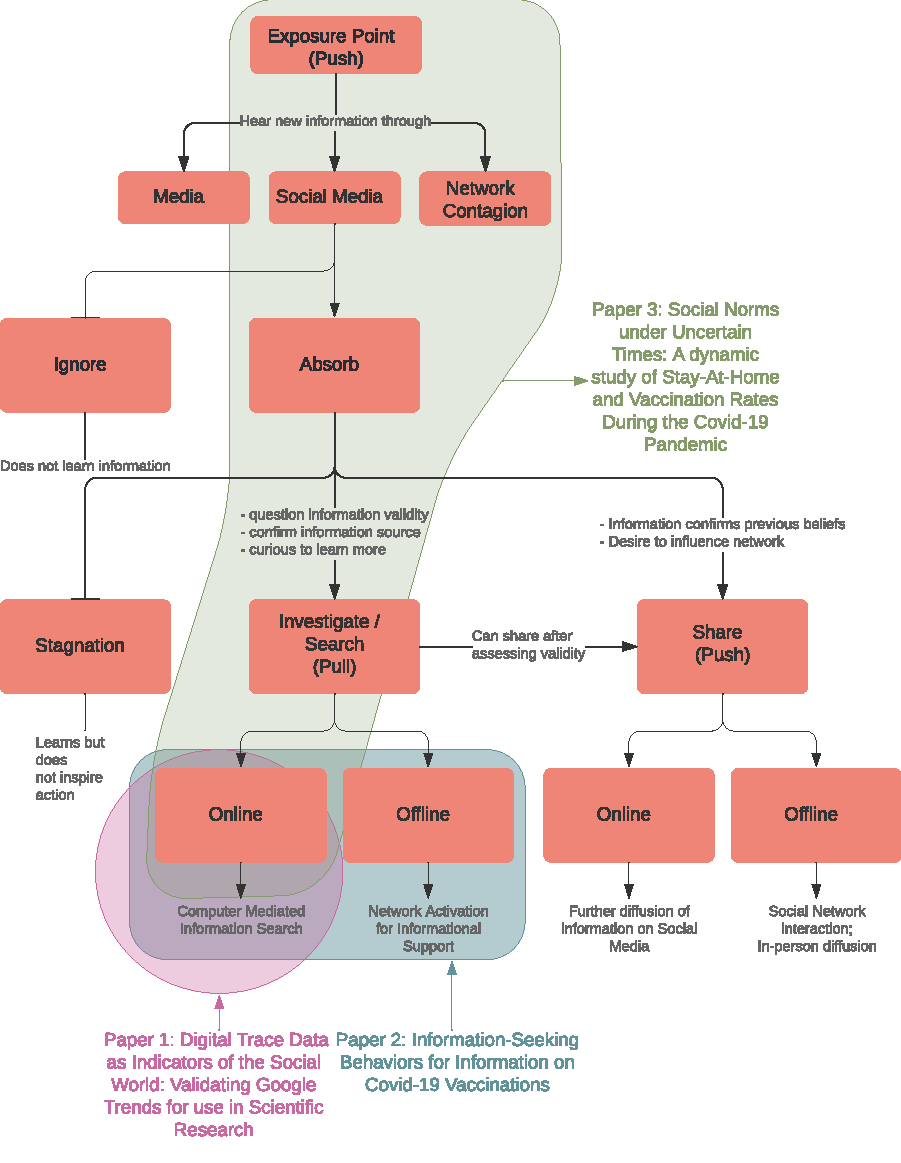
\includegraphics[width=\linewidth]{figs/ch1/Dissertation Concept Map - Color.pdf}}
\caption{Theoretical Framework for the Dissertation}\label{fig:concept-map}
\end{figure}

To make my intended contributions to the literatures on computational
social science, sociological methodology, social norms, social networks,
and diffusion, my dissertation will take the following format:

\subsection{Article 1: Construct Validity and Correspondence of Google Trends}
% TODO Double check name
% TODO link to article  
I will first investigate how Google Search Trends can be operationalized
as cultural attitudes, disease prevalence and voting behaviors through
comparing trends data to observed valid indicators of these cases.
Specifically, I will test cultural indicators from the NORC General
Social Survey, United States county-level suicide rates from National
Center for Health Statistics, US case rates of Covid-19 from The New
York Times, historical US Presidential Election results, and the
American National Election Survey against selected Google Trends terms
and analyze the data using correlation methods. The aim of this article
is to assess the construct validity and will contribute to critical big
data studies and sociological methodology.
% TODO ADD IN ARTICLE 1 ABSTRACT

\subsection{Article 2: Information-Seeking Behaviors for Information on Covid-19 Vaccinations}
% TODO Double check name
% TODO link to article  
The second article in my dissertation investigates the question "what
are the behavioral processes that lead to macro-level outcomes" (in this
case, Google Trends results) proposed by \citet{breigerScaling2015}. Knowing that
Google trends data only encompasses a small portion of the
information-seeking done by modern humans, it is important to
investigate what leads individuals to search for a question online using
a search engine (contributing to macro-level trends data) versus more
traditional means of information gathering, such as network activation
(asking someone in their social network for informational support). To
investigate this, I use the case of receiving, requesting, and sharing
information about the Covid-19 vaccine in a survey I received funding to
conduct of 900 Adults in the United States.

Previous research has greatly failed to distinguish between the activation of
information seeking behaviors online and offline. Using theories of social
support and uses and gratifications theory I investigate the factors associated
with each vehicle type when on information seeking vehicle: personal connection,
doctor, social networking site, online forum, and online search engine. Using
novel survey data of % TODO  nrow(rain) Americans and their experience seeking out
information about the Covid-19 vaccines, I find little evidence that online
search is more utilized than seeking social support from personal network
connections or health professionals. I find evidence that the vehicles queried
in this survey are conceptually different and that the utilization of different
vehicles varies by demography and information sources. Finally, I find that
different fountains of information and information search vehicles hold real
world consequences through their associations with Covid-19 vaccination rates
and intentions, as information from a doctor increased the Covid-19 vaccination
uptake while receiving information from a Social Networking Site like Facebook
or Twitter was associated with lower odds of vaccination.  

\subsection{Article 3: Social Norms under Uncertain Times: A dynamic study of Stay-At-Home and Vaccination Rates During the Covid-19 Pandemic}
% TODO Double check name
% TODO link to article  
My final article takes a deeper dive into the formation of social norms
governing health behaviors in cases of extreme uncertainty using the
cases of both a) population mobility during early 2020 and b)
vaccination rates during early 2021, both as responses to public health
recommendations to mitigate the Covid-19 pandemic. Using theories of
associative diffusion and the integrated theoretical framework of norms,
I test how these health behaviors are outcomes of assortative signaling
from networks and other sources, such as social isolation and connection
between communities, religious and political conservativism, and
attention to media sources, and online norms as measured by
information-search behaviors. To investigate this, I conduct statistical
modelling on a dataset I compiled from multiple sources, including
Google, Facebook, and the Center for Disease Control and Prevention.

This paper examines how social norms are formed under conditions of uncertainty
using the case studies of stay-at-home and vaccination rates during the Covid-19
pandemic.  I test fear-based models of behavioral adaption to public health
recommendations as well as patterns of complex social contagion using linear
mixed effects models. These models show that complex contagion is a valid
framework for the social contagion of new norms during Covid-19. However, I find
important moderating effect of signal discordance, the contextual diversity of
signals received by an ego.
